%\emph{\emph{•}}
\documentclass{llncs}
%
\usepackage{amsmath}
\usepackage{amsfonts}
\usepackage{amssymb}
\usepackage{graphicx}
\usepackage{subcaption}
\captionsetup{compatibility=false}
\usepackage{url}
\usepackage[usenames]{color}

\newcommand{\keyterms}[1]{\par{\bfseries{ Key Terms: }}#1}

\begin{document}
\title{Distributed Datastores: Consistency Metric for Distributed Datastores}
\author{Kyrylo Rukkas\and Galyna Zholtkevych}
\institute{V.N.~Karazin Kharkiv National University\\
	4, Svobody Sqr., 61022, Kharkiv, Ukraine\\
	\email{galynazholtkevych1991@gmail.com}}
\maketitle
\begin{abstract}
Distributed databases being evolved require write requests to be handled independently to increase availability.
This means that nodes in a database can process modifying operation. This involves huge conflicts and leads to
full inconsistency and mess between replicas. This paper investigates a trade-off between availability and consistency
in a distributed database.
\end{abstract}

\section{Introduction}\label{sec:intro}
In the epoch of popular usage of IoT, Big Data, Cloud Computing, the data become more and more
important thing and require larger, more reliable storage. This leads to increasing size of distributed
storages. They become bigger and bigger and require the huge network across all the distributed nodes.
But there are several unsolved problems using large distributed datastores and some of them are strongly related
to the CAP-theorem. Given that the ACID strategy can not be supported for systems of this class \cite[{\color{red} references to the CAP-conjecture})]{?}, mechanisms for delivering data across distributed storage still lack fast consistency convergence, reliability and tolerance to network partitions.
{\color{red}
Provide facts for this problem. (links etc.)
}


Supporting replicas of an evolving distributed system up-to-dates is very important but hard problem. Thus we need to provide a set of indicators of main characteristics of the distributed data store to assess the risk of a wrong decision because of the data inconsistency or unavailability.
In this paper, we focus our study on the problem of estimating data consistency in a distributed data store.

Given that in a distributed data store consistency of replicas may only be eventually \cite[{\color{red} you need to refer to the corresponding papers}]{?}, we need the answering the following questions
\begin{enumerate}
\item
How to resolve conflicts between replicas?
This problem is raised and partially solved in \cite{bib:c_ts}, where algorithm with timestamps on replicas is proposed.
But merging updated replicas, it takes the response time, so consistency convergence decreases.
In the paper further sections we will investigate faster consistency convergence.
\item
Is it always possible to ensure the convergence to the consistency of data and by what means can this be achieved?
This depends on many factors including network topology,
network failures, links bandwidth, bottlenecks in network overall etc \cite[{\color{red} links are needed}]{?}.
\item
What methods can be used to effectively solve the broadcast storm problem?
This is well-known problem and it has the solution in \cite[{\color{red} links are needed}]{?}.
\item How do loops when broadcasting data be eliminated?
This is what networking algorithms aimed to solve \cite[{\color{red} links are needed}]{?}.
\end{enumerate}

\section{Evolving consistency metric mathematical model: Derived metrics}

In the previous paper {\color{red} Link to paper} we considered the metrics for all three elements of CAP-theorem.
Now our paper is mainly devoted to consistency question and how fast it can converge.
From previous paper we are taking the developed mathematical model.
(Refresh model here, specify only needed elements - nodes, dataunits, replicas)
$N$ - ....
$N(d)$ - the set of nodes that are having given dataunit $d$.
$l(N(d))$ - the number of nodes in datastore that are having given dataunit.

Let us continue forming this model.
Our mathematical model for consistency $C$ will be able to define the time which distributed datastore require
to become fully consistent. Also let's denote  $IC$ as a value calculated by probabilistic formula for the number of compare operations that should be done for each pair of nodes to find inconsistency.
Obviously, if the storage is consistent, the number of operations will be the maximum. It will allow to calculate the upper, lower boundary, average number of steps could be taken to find if the system is consistent or not.
In this paper our mathematical model for consistency $C$ will be able to define inconsistency degree in a given datastore (see Case study subsection), and afterwards will focus on time which distributed datastore require to become fully consistent and some other helpful metrics (see subsections ...)


\subsection{Case Study}\label{sec:experiments}

Let's denote  $IC$ as a value calculated by probabilistic formula for the number of compare operations that should be done for each pair of nodes to find inconsistency.
Obviously, if the storage is consistent, the number of operations will be the maximum.
Then the model will allow to calculate the upper, lower boundary, average number of steps could be
taken to find if the system is consistent or not.
We are thinking that having this formula will help us to eventually fully specify the mathematical model for consistency, so let it be one of mathematical model components. Let's claim some rules that can help to investigate
consistency.


{\color{red} Prove that having random topology the best algorithm to allocate masters and slaves
in the next manner: each master has those neighbors-slaves that are closest to it comparing
other master nodes.}

Based on proposed hypothesis we want to check ... .
So the probability of that two nodes taken at random are from consistent subset is

$p = \frac{n_c}{l(N_d)} * \frac{n_c - 1}{l(N_d) - 1} = \frac{n_c * (n_c - 1)}{l(N_d)* (l(N_d) -1)}$ where $n_c$ is the number of consistent nodes in the system at initial time $t$ (when we block the system and start investigating).

Obviously, inconsistency probability then:

$p_{ic} = 1 - p = 1 - \frac{n_c * (n_c - 1)}{l(N_d)* (l(N_d) -1)}$
Taking into account that minimum number of consistent nodes will be equal to 1, and the maximum number of consistent nodes is equal to $l(N_d)$, we have following consequences:
\begin{itemize}
\item The system is fully consistent if $p = l(N_d) / l(N_d) = 1$
\item The lower boundary for consistency probability is $1 / l(N_d)$
\end{itemize}

We developed the consistency formula for two nodes. Let's now extend it to more general one.
We still suppose that a data unit is represented by replicas on $N_d$ servers. Let's denote it as temporary $N$.
Let we have $K$ classes of mutually consistent replicas.
Then we denote by $N_k$ a number of replicas in $k^\mathrm{th}$ consistency class ($1\leq k<K$).
It is evident that $N_k>0$ for all $k=1,\ldots,K$ and $N=N_1+\ldots+N_K$.
Such representations $N=N_1+\ldots+N_K$ are called integer partitions.

\noindent Thus, in this case any integer partition describes some inconsistency state.

\begin{example}\label{ex:partitions}
All integer partitions for $5$ are
\begin{center}
\begin{tabular}{lclcl}
	5 & & 4+1 & & 3+2\\
	3+1+1 &\hspace*{10pt}& 2+2+1 &\hspace*{10pt}& 2+1+1+1\\
	1+1+1+1+1
\end{tabular}
\end{center}
\end{example}

Taking into account this consideration we define inconsistency metric for a data unit in the term of the corresponding integer partition.
More details, let us suppose that the studied data unit $u$ is represented by $N$ replicas, which are being described by the integer partition $N=N_1,\ldots,M_K$ then the inconsistency metric $I(u)$ is defined by the formula
\begin{equation}\label{eq:metric}
	I(u)=1-\sum_{k=1}^K\dfrac{N_k(N_k-1)}{N(N-1)}.
\end{equation}

\begin{example}\label{ex:metric}
Let us suppose that a data unit $u$ are being stored on five servers.
Then the corresponding inconsistency states (see Example~\ref{ex:partitions}) have the following values of the inconsistency metric
\begin{center}
\begin{tabular}{lclcl}
	$I(5)=0$ & & $I(4+1)=\frac{2}{5}$ & & $I(3+2)=\frac{3}{5}$\\
	$I(3+1+1)=\frac{7}{10}$ &\hspace*{10pt}& $I(2+2+1)=\frac{3}{4}$
		&\hspace*{10pt}& $I(2+1+1+1)=\frac{9}{10}$\\
	$I(1+1+1+1+1)=1$
\end{tabular}
\end{center}
The meaning of $I(u)$ is the value of probability to establish the fact of inconsistency by the way of comparison two randomly chosen replicas.
\end{example}
Example~\ref{ex:metric} demonstrates that the proposed metric is equal to $0$ for the absolutely consistent data unit (the case 5) and is equal to $1$ for the absolutely inconsistent data unit (the case 1+1+1+1+1).

This study had been checked by the following experimentation: we implemented a code that allows to test the accuracy of the inconsistency model described above. Partitions probability intervals for different partitions are demonstrating that the formulae is correct. To be more intuitive we took the same number of nodes and same partitions.

It is obviously that we do not have exact matching, because the experiment is based on number of iterations where two random nodes are taken from a set of nodes and we count them consistent if they are in the same partition.
It is also obvious that for one consistent partition inconsistency will be equal $0$ and for maximum number of consistent partitions the inconsistency will be equal to $1$.

\begin{figure}
\begin{subfigure}{0.5\linewidth}
\centering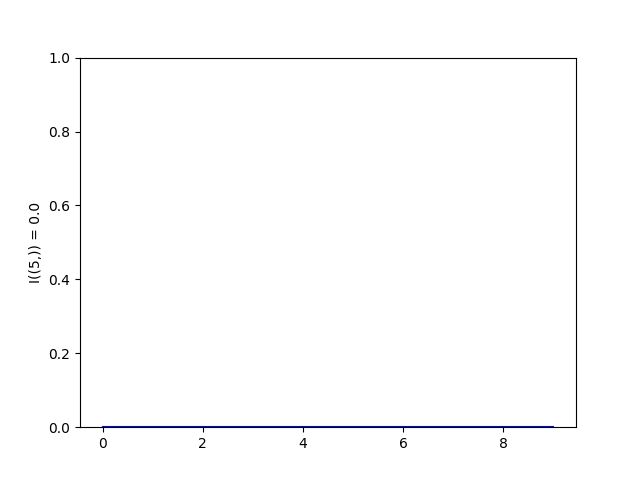
\includegraphics[scale=0.4]{images/1-consistent-partition.png}\hfill
\end{subfigure}
\begin{subfigure}{0.5\linewidth}
\centering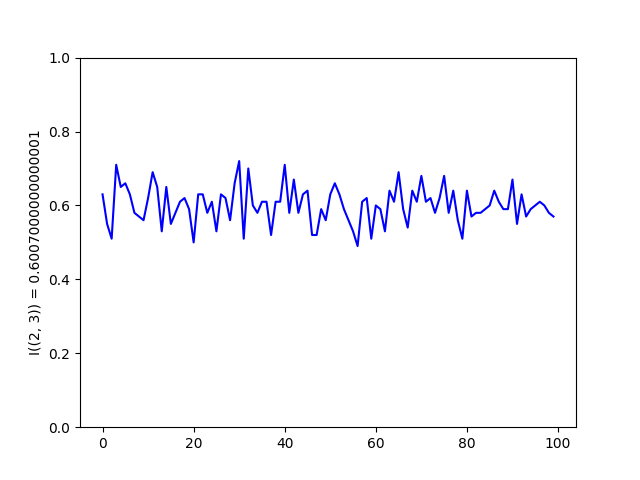
\includegraphics[scale=0.4]{images/2-3-consistent-partitions-probability.png}\hfill
\end{subfigure}
\begin{subfigure}{0.5\linewidth}
\centering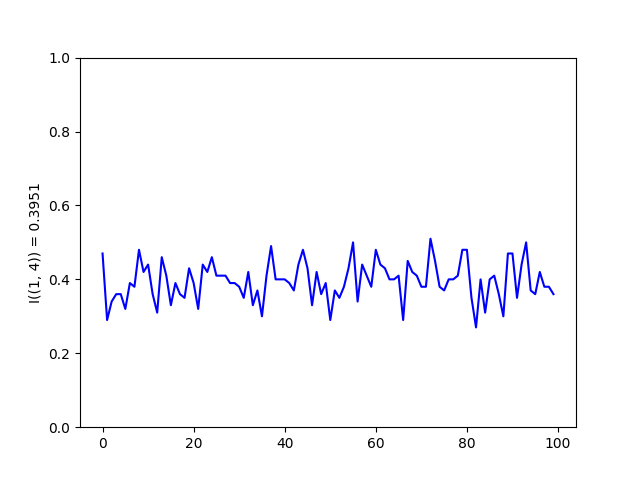
\includegraphics[scale=0.4]{images/1-4-consistent-partitions-probability.png}
\end{subfigure}
\begin{subfigure}{0.5\linewidth}
\centering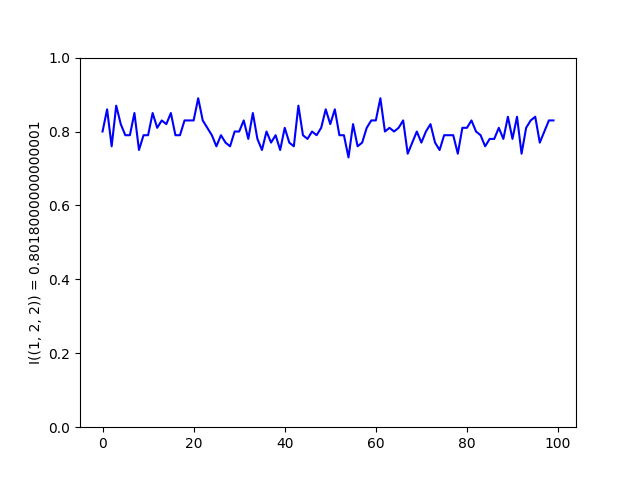
\includegraphics[scale=0.4]{images/1-2-2-consistent-partitions-probability.png}
\end{subfigure}
\begin{subfigure}{0.5\linewidth}
\centering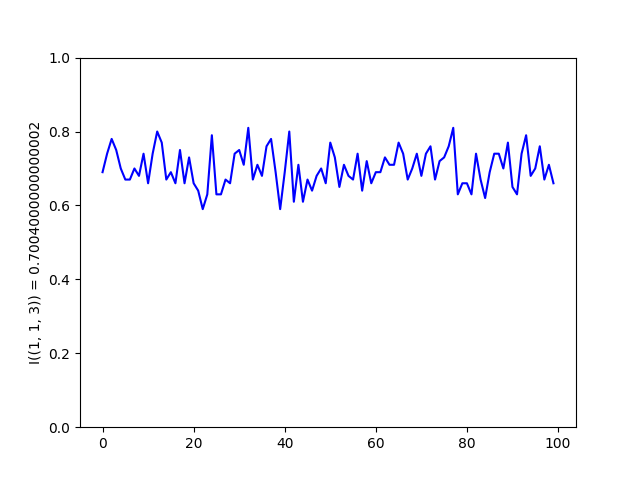
\includegraphics[scale=0.4]{images/1-1-3-consistent-partitions-probability.png}
\end{subfigure}
\begin{subfigure}{0.5\linewidth}
\centering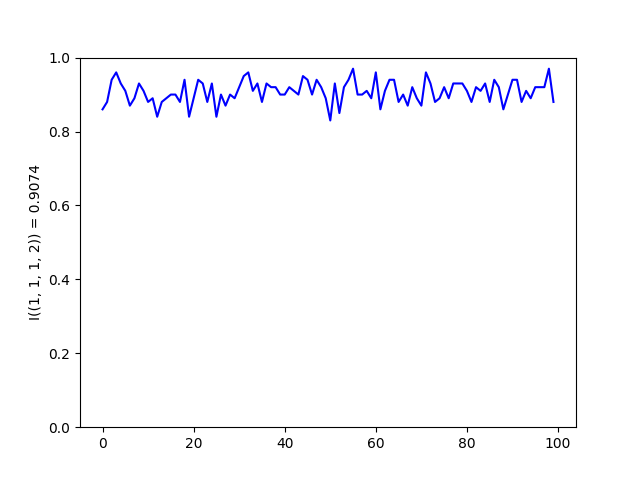
\includegraphics[scale=0.4]{images/1-1-1-2-consistent-partitions-probability.png}
\end{subfigure}
\end{figure}

\newpage

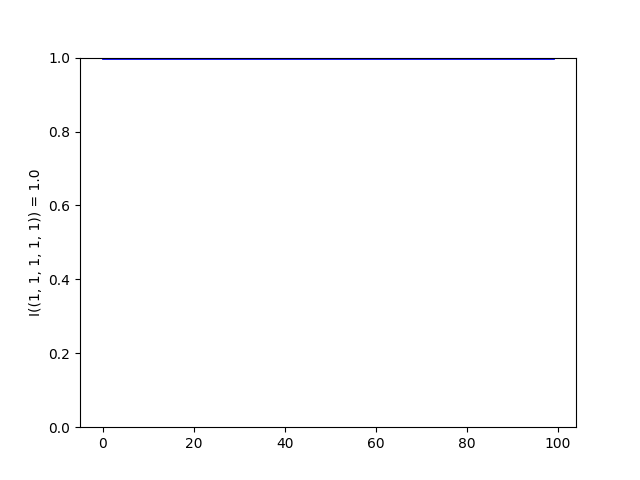
\includegraphics[scale=0.4]{images/1-1-1-1-1-consistent-partitions-probability.png}

\section{One Metric to Assess Consistency of Data}
{\color{red} This metric is derived and studied in case study, so this subsection is not needed anymore}
\section{Simulation Model to Assess Inconsistency Ratio of Data}
{\color{red} Should come in the end as annex}

\subsection{Consistency probability}

We want to calculate the maximum number of compare operations to find inconsistency. Let us imagine that the datastore is fully consistent. This will require comparing all nodes with each other.

We also assume that one of two nodes to be compared are taken randomly except of already taken ones. So the algorithm is the following at first iteration we take two nodes at random, put out one of them if they are consistent and continue comparing with randomly taken nodes. Once we have two inconsistent nodes, the comparing ends.

We have two types of events in such a system: two chosen nodes are consistent or two nodes are inconsistent.
Assume that $p$ is the probability that two nodes are consistent, and
$q = 1 -p$ - the probability that two nodes are inconsistent.
$l(N_d)$
Then our sample space looks like:

$\Omega = \{q, qp, qp^2, ..., qp^n\}$

Then the number of comparing operations is:

$\vert\Omega\vert = \sum_{i=0}^{l(N_d)-1}qp^i$

From this formulae we have next constraints:
\begin{itemize}
\item The system is fully consistent if $\vert\Omega\vert = l(N_d)-1$
\item The system is inconsistent when $1 <= \vert\Omega\vert <= l(N_d) -2$
\end{itemize}

Thus, in the end probability that the node is consistent at time t will be equal to number of consistent nodes (nodes with newest replica versions) $/ l(N_d)$, where $l(N_d)$ is the current length of subset $N_d$ (taking in account that each iteration we put put one node)

\subsection{Convergence time complexity}


Now we are interested to calculate the time that can be taken for consistency convergence.
Let it be the trivial network where all links have capacity 1. Then each edge of graph has weight 1.
Let's imagine the nodes that are at the largest distance each from other. In the distributed datastore nodes are
broadcasting each to other in parallel. So the upper boundary of consistency in the worst case is the maximum of
shortest paths. It is well-known that this is diameter of the graph:


$n_ts = diameter(G)$.


Let's imagine now the real topology where the network graph topology is weighted.
Let the diameter be the path:


$P = [e_1....e_n]$, where $e_i$ has own weight.


Then time taken for consistency to converge is:

$\sum_1^{n}w_i$ where $w_i$ is the weight of $i$ edge of the path $P$.


\subsection{Replica's actuality research}

Let's also measure the number of steps to find the degree of consistency at a time $t$.
Our algorithm described above is complemented by that fact that if we find inconsistent nodes,
we are taking the node with latest replica timestamp. At each node meeting replica version equal to current maximum, we accumulate the count of such nodes. The count is dropped when the new current maximum is found. This is actually the algorithm of search of maximum number in a sequence and has known complexity - $O(N)$ comparisons.
Then, in our case it is $O(l(N_d))$ steps.



\section{Remained studying}\label{sec:experiments}

Экспериментальное исследование.
1. Смоделировать граф с нодами разной консистентности и вычислить среднее кол-во тайм слотов, которое может быть потрачено на нахождение inconsistency. - to be studied more. Мы вычислили вероятность, а не время consistency convergence. Выполнено на 50%

Привести экспереименты с 2, 3, 4 разбиениями

2. Показать когда система полностью консистентна - выполнено

3. Показать, что приведение системы к консистентности - это кол-во тайм слотов от (1, диаметра графа). - выполнено

4. Нахождение самой актуальной реплики и кол-во консистентных ей - сколько тайм слотов - выполнено

Investigation what is better for fast consistency convergence:
group of masters close enough each to other (this almost replaces centralized server)
or group of masters allocated in far each from other but having close at least one of slaves.

This needs statistic experiment

\section{Inconsistency metric in various kinds of algorithms spreading replicas across DDS}
Все исследования сейчас основываются на предположении абсолютной надежности сети (отсутсвие network partitions) и отсутствие ограничений на пропускную способнсть (капасити линков равное единице).

Вычислить на основе иммитационных экспериментов на графе метрику инконсистентности на разных алгоритмах (эпидемический).

\section{Different topologies}
- Полносвязный граф
- Регулярный граф
- Рандомный граф

- Граф, где писать нужно на определенные узлы (мастера). Проверить идею, насколько она лучше других, когда у каждого мастера есть примерно по одинковому кол-ву соседей - слейвов (Один слейв может быть соседом несколкьих мастеров, это не есть ограничением). Сравнить с вариантом, когда мастера сгруппированы в одном месте (сходится к ситуации централизованного хранилища и не имеет смысла). И с вариантом, когда мастера отдаленно друг от друга, а слейве где попало.
Внедрить разное капасити (edge weight) для линков.

\section{Future work}
!!!! Отдельная секция про availability или на дальнейший ресерч -

Алгоритм распространения-очищения реплик. Если даатаюнит часто запрашивается, то реплика его появляется там, где он часто запрашивается. Когда таймаут запроса к нему истечет (он больше не интересен), реплика его удаляется с этого места.
Исследовать, насколько может повыситься consistency и availability.

- Внедрить возможность когда показатели надежности падают, network partitions возникают.


\section{Conclusion}

\begin{thebibliography}{00}

\bibitem{bib:c_ts}
Sanjay Kumar Madria: 
Handling of Mutual Conflicts in Distributed Databases using Timestamps,
The Computer Journal. Vol. 41, No.\,6 (1998) 

\bibitem{bib:andrews}
Andrews,~G.\,E.:
The theory of partitions.
Addison-Wesley (1976)
\end{thebibliography}
\end{document}

